\documentclass{ximera}
\input{../preamble}
\addPrintStyle{..}

\begin{document}
	\author{Zomercursus KU Leuven}
	\xmtitle{Optellen en vermenigvuldigen}{}
	\label{xim:cmplx_optellen_en_vermenigvuldigen}



    Optelling en vermenigvuldiging van complexe getallen volgen uit de gebruikelijke rekenregels.
    Je mag en moet wel steeds $i^2$ vervangen door $-1$, zodat de uitkomsten steeds kunnen geschreven worden in de \textit{standaardvorm} $a+bi$. 
    
    \begin{definition}[Som en product] Voor reële getallen $a,b,c,d$ geldt door uitwerken en $i^2=-1$ dat

    \formulevb{(a+bi)+(c+di) = (a+c)+(b+d)i}{(1+2i) + (3+4i) = (1+3) + (2+4)i = 4+6i}

    \formulevb{\begin{array}{@{ }r@{ }l@{ }}(a+bi) \cdot (c+di) & = ac + adi+ bci+ bdi^2 \\ &  = (ac -bd) + (ad+bc)i\end{array}}{{\begin{array}{@{ }r@{ }l@{ }}(1+2i) \cdot (3+4i) & = 1\cdot3 + 1\cdot4i+ 2\cdot3i+ 2\cdot4i^2 \\ &  = (3 - 8) + (4+6)i \\ & = -5+10i\end{array}}}
    
    \end{definition}

    \begin{example}\nl
        \begin{xmmulticols}
        \begin{question}$(2-4i) + (3+5i)  = \answer[onlineshowanswerbutton]{5+i}$ 
            \begin{feedback}[correct]\nl
                $(2-4i) + (3+5i) = 2 -4i + 3 + 5i = 2 + 3 -4i +5i = 5 - i$
            \end{feedback}            
        \end{question}
        \begin{question}$(3+i) - (1-2i)   = \answer[onlineshowanswerbutton]{2+3i}$ 
        \begin{feedback}[correct]\nl
            $(3+i) - (1-2i)  = 3 + i - 1 + 2i = 3 - 1 + i + 2i = 2 + 3i$
        \end{feedback}	
        \end{question}
        \begin{question}$(3+i) \cdot (1-2i)   = \answer[onlineshowanswerbutton]{5-5i}$ 
        \begin{feedback}[correct]\nl
            $(3+i) \cdot (1-2i)  = 3\cdot1 + 3\cdot(-2i) +i\cdot 1 + i\cdot(-2i) = 3-6i+i-2i^2$ $=3-5i-2\cdot(-1)   =  3-5i + 2 = 5-5i$
        \end{feedback}	
        \end{question}
        \begin{question} $(1-i)+(2+i)   =\answer[onlineshowanswerbutton]{3}$     \end{question}
        \begin{question} $(-3+2i)+(3+5i)=\answer[onlineshowanswerbutton]{7i}$    \end{question}
        \begin{question} $(-3+2i)i      =\answer[onlineshowanswerbutton]{-2-3i}$ \end{question}
        \end{xmmulticols}
    \end{example}
            

  De som van complexe getallen komt overeen met de som vectoren via de parallellogramregel:

    \begin{image}[0.8\textwidth]
        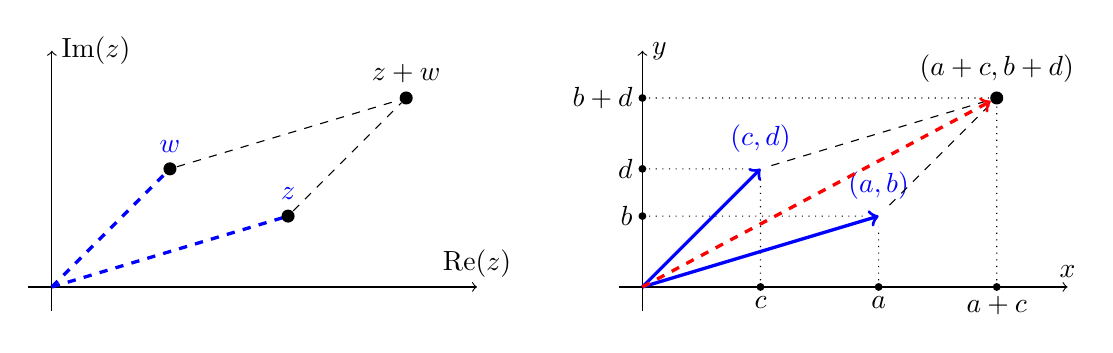
\begin{tikzpicture}[scale=3]%,cap=round,transform canvas={scale=0.5}]
        
        \draw[->] (-0.1,0) -- (1.8,0) node[above] {Re$(z)$};
        \draw[->] (0,-0.1) -- (0,1)   node[right] {Im$(z)$};
        
        \draw[color=blue,very thick,dashed] (0:0)  -- (1,0.3) node[black, name=Z1,circle, fill=black, radius=1pt,scale=0.5] {} node [yshift=2pt,above] {$z$}; 
        \draw[color=blue,very thick,dashed] (0:0)  -- (0.5,0.5) node[black, name=Z2,circle, fill=black, radius=1pt,scale=0.5] {} node [yshift=2pt,above] {$w$}; 
        
        %
        \draw[color=black] (1.5,0.8) node[name=Zs,circle, fill=black, radius=1pt,scale=0.5] {} node [yshift=2pt,above] {$z+w$} ;  
        %
        % \draw[dashed] (1,0)    node[circle, fill=black, radius=1pt,scale=0.3] {} node[below] {$a$} -- (Z1);
        % \draw[dashed] (0,0.3) node[circle, fill=black, radius=1pt,scale=0.3] {} node[left] {$b$} -- (Z1);
        % %
        % \draw[dashed] (0.5,0) node[circle, fill=black, radius=1pt,scale=0.3] {} node[below] {$c$} -- (Z2);
        % \draw[dashed] (0,0.5)   node[circle, fill=black, radius=1pt,scale=0.3] {} node[left] {$d$} -- (Z2);
        % %	
        % \draw[dashed] (1.5,0)    node[circle, fill=black, radius=1pt,scale=0.3] {} node[below] {$a+c$} -- (Zs);
        % \draw[dashed] (0,0.8) node[circle, fill=black, radius=1pt,scale=0.3] {} node[left] {$b+d$} -- (Zs);
        % %
        \draw[black, dashed] (Z1) -- (Zs);
        \draw[black, dashed] (Z2) -- (Zs);
    
        \begin{scope}[xshift=2.5cm]
        \draw[->] (-0.1,0) -- (1.8,0) node[above] {$x$};
        \draw[->] (0,-0.1) -- (0,1)   node[right] {$y$};
    
        \draw[color=blue,very thick,->] (0:0)  -- (1  ,0.3)  node [name=Z1]{} node[yshift=2pt,above] {$(a,b)$}; 
        \draw[color=blue,very thick,->] (0:0)  -- (0.5,0.5)  node [name=Z2]{} node[yshift=2pt,above] {$(c,d)$};
        %
        \draw[color=black] (1.5,0.8) node[name=Zs,circle, fill=black, radius=1pt,scale=0.5] {} node [yshift=2pt,above] {$(a+c,b+d)$} ;  
        %
        \draw[dotted] (1,0)    node[circle, fill=black, radius=1pt,scale=0.3] {} node[below] {$a$} -- (Z1);
        \draw[dotted] (0,0.3) node[circle, fill=black, radius=1pt,scale=0.3] {} node[left] {$b$} -- (Z1);
        %
        \draw[dotted] (0.5,0) node[circle, fill=black, radius=1pt,scale=0.3] {} node[below] {$c$} -- (Z2);
        \draw[dotted] (0,0.5)   node[circle, fill=black, radius=1pt,scale=0.3] {} node[left] {$d$} -- (Z2);
        %	
        \draw[dotted] (1.5,0)    node[circle, fill=black, radius=1pt,scale=0.3] {} node[below] {$a+c$} -- (Zs);
        \draw[dotted] (0,0.8) node[circle, fill=black, radius=1pt,scale=0.3] {} node[left] {$b+d$} -- (Zs);
        %
        \draw[black,dashed] (Z1) -- (Zs);
        \draw[black,dashed] (Z2) -- (Zs);
        \draw[red,very thick, dashed,->] (0,0) -- (Zs);
    
        \end{scope}
        %
        % onzicktbaar: enkel voor alignment met vorige picture !
        %\path [thick, red,decorate,decoration={brace,amplitude=10pt,mirror},yshift=-5pt](0,0) -- (1,0) node[black,midway,yshift=-0.6cm] {};
        
        \end{tikzpicture}
    \end{image}

    Net zoals bij de reële getallen spreken we ook van het \textbf{tegengestelde}  $-z=-(a+bi)= -a-bi$.
    
    De vermenigvuldiging heeft een wat ingewikkeldere meetkundige interpretatie die \hyperref[TODO]{elders} wordt uitgelegd.
    
    
    \begin{exercise} \nl 
        %	\begin{xmmulticols}

            \begin{question}$(1+2i) \cdot (1-2i) = \answer[onlineshowanswerbutton]{5}$ 
            \begin{oplossing}\nl
            Haakjes uitwerken, of eenvoudiger via $(a-b)(a+b) = a^2 - b^2$ wat ook geldt voor complexe getallen:
            $$
            (1+2i) \cdot (1-2i) = 1^2 - (2i)^2 = 1 + 4 = 5
            $$
            \end{oplossing}	
            \end{question}
            \begin{question}$(1+2i) \cdot \frac{1-2i}{2} = \answer[onlineshowanswerbutton]{\frac52}$ \end{question}
            \begin{question}$(1+2i) \cdot i = \answer[onlineshowanswerbutton]{-2+i}$ \end{question}
            \begin{question}$i^3 = \answer[onlineshowanswerbutton]{-i}$
            \begin{oplossing}
            $i^3 = i\cdot i^2 = -i$
            \end{oplossing}    
            \end{question}
            \begin{question}$i^4 = \answer[onlineshowanswerbutton]{1}$
            \begin{oplossing}
            $i^4 = i^2\cdot i^2 = (-1) \cdot (-1) = 1$ of $i^4 = (i^2)^2 = (-1)^2 = 1$
            \end{oplossing}    
            \end{question}
        %	\end{xmmulticols}
        \end{exercise}
        
\end{document}

